\chapter{Experiment}
\section{Single Joint Examples}\label{sec:simpleExamples}
This section contains step by step examples of how my system functions properly with the hubo system allowing for multiple processes to work with the system

	\subsection{Joint Space Step Response}\label{sec:singlejointStep}
		This section shows the experimental and expected results of controlling a single joint via the Hubo-Ach system.
In this example the right shoulder pitch (RSP) is given a step input from 0.0 $rad$ to 0.4 $rad$.
The reference position $\theta_r$ is begin recorded as well as the actuator setpoint $\theta_c$ and the actual position of the joint $\theta_a$.
These definitions are also available in Table~\ref{table:recorded}

\begin{table}
\centering
\caption{States being recorded for the single joint step response test}
\begin{tabular}{l || c | c | c | c}
Signal      & Symbol     & Definition                    & Source      & Units \\
\hline
\hline
FeedForward & $\theta_r$ & Desired reference on the      & Hubo-Ach   & $rad$ \\
            &            & Hubo-Ach FeedForward Channel  &            &       \\
\hline
FeedForward & $\theta_c$ & Reference set to the actuator & Hubo-Ach   & $rad$ \\
\hline
Feedback    & $\theta_a$ & Actual position of joint as   & JMC        & $rad$ \\
            &            & measured from the encoders    &            &       \\
\hline
\end{tabular}
\label{table:recorded}
\end{table}



\begin{figure}[thpb]
  \centering
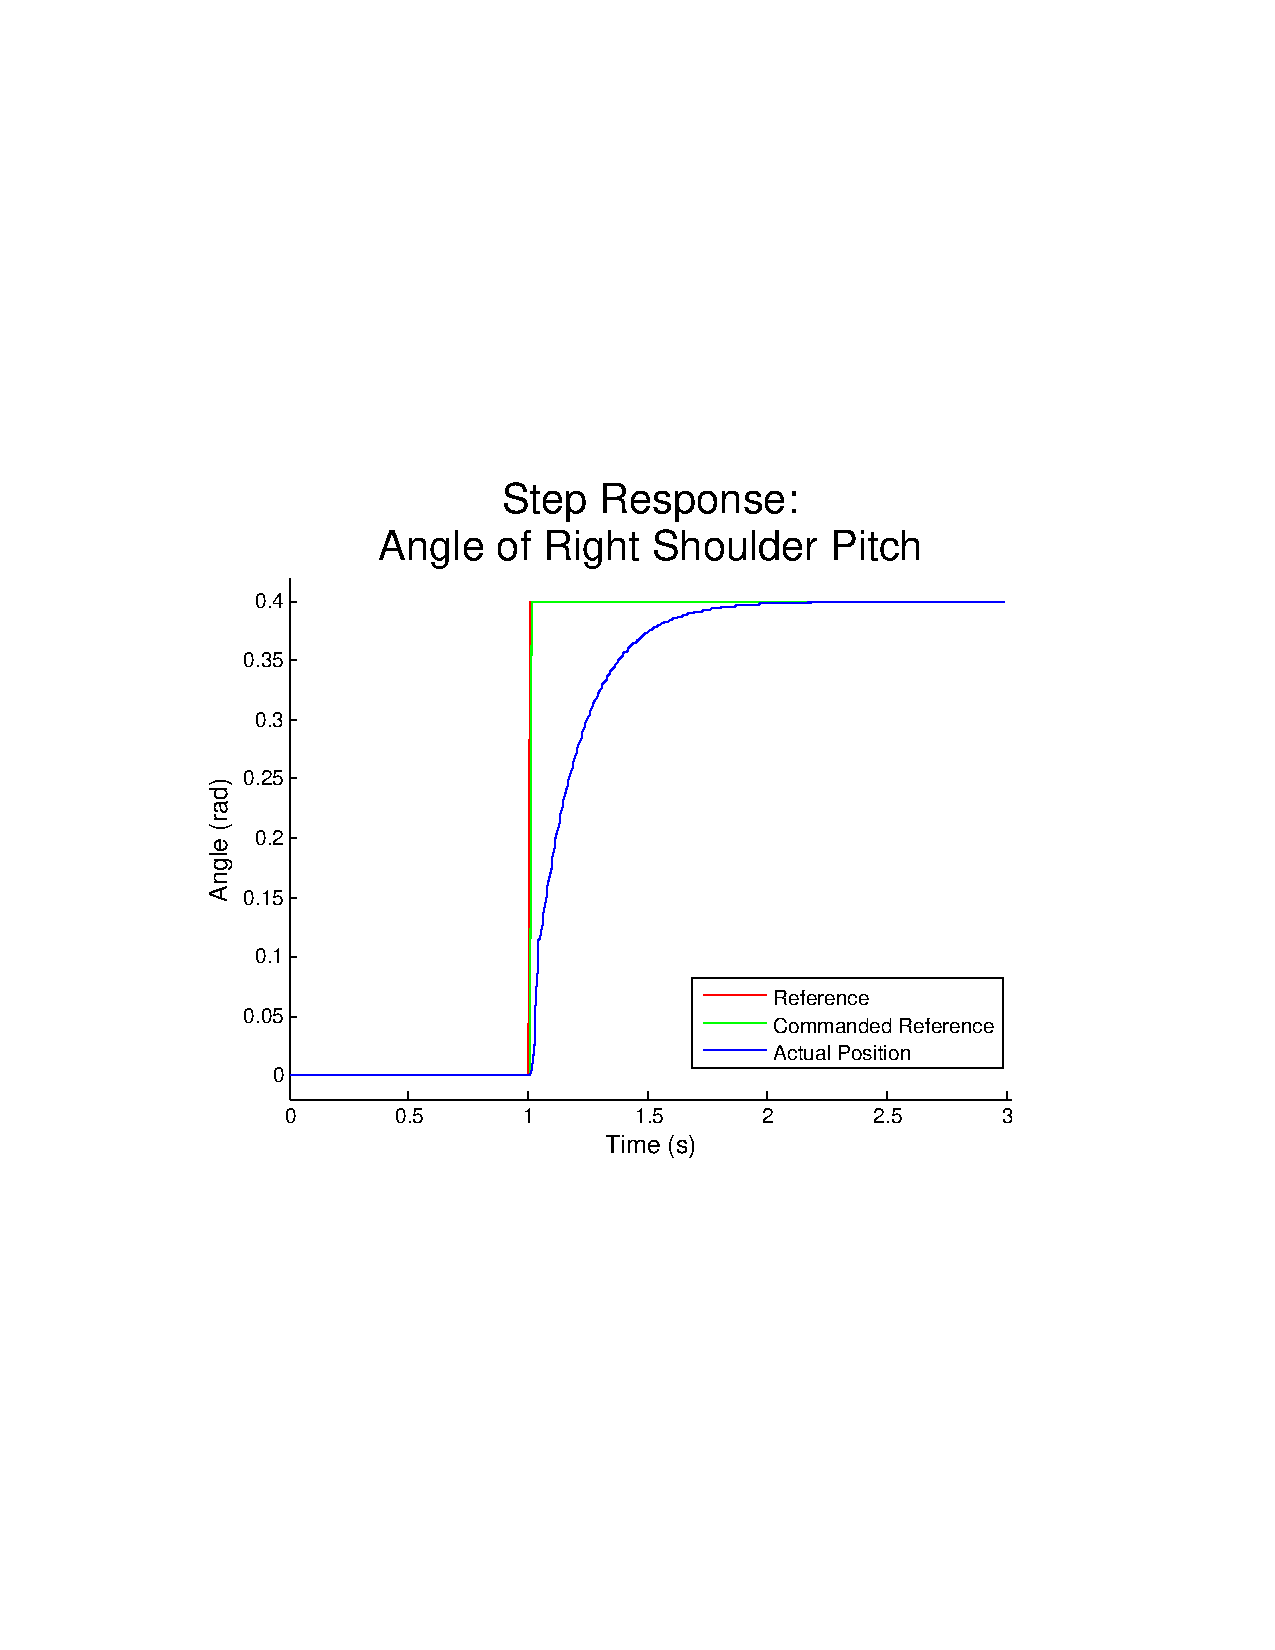
\includegraphics[width=0.8\columnwidth]{./examples/pix/RSP-Zp4-step-step-crop.pdf}
  \caption{The commanded reference plotted against the actual reference recorded via Hubo-Ach and ground truth via CAN analyzing utilities.  In this plot the commanded reference is not automatically filtered by Hubo-Ach.  The commanded joint is the right shoulder pitch.}
  \label{fig:singleJointStep}
\end{figure}

Fig.~\ref{fig:singleJointStep} shows the results when a step input is applied and Hubo-Ach is in \textit{HUBO\_REF\_MODE\_REF\_FILTER} also know as pass-through mode.
This sets the what the desired reference on the \textbf{FeedForward} Hubo-Ach channel to the actuator's reference, i.e.:

\begin{equation}\label{eq:refrefmode}
 \theta_c(N) = \theta_r(N)
\end{equation}

Fig.~\ref{fig:hubo-ach-feedforward} shows the block diagram of the control setup.

\begin{figure}
\centering
\begin{tikzpicture}[->,>=stealth',shorten >=1pt,auto,node distance=5cm,
  thick,main node/.style={fill=white!20,draw,font=\sffamily\Large\bfseries}]


  \node[main node] (ref) {Reference};
  \node[main node] (hubo-ach) [right of=ref] {Hubo-Ach};
  \node[main node] (hubo) [right of=hubo-ach] {Hubo};




  \path[<->,dashed, every node/.style={font=\sffamily\small}]
    (hubo) edge node [above] {CAN} (hubo-ach);

  \path[->,every node/.style={font=\sffamily\small}]
    (ref) edge node [above] {$\theta_r$} (hubo-ach);


\end{tikzpicture}
\caption{Reference $\theta_r$ being applied to Hubo via Hubo-Ach.  $\theta_r$ is set on the \textbf{FeedForward} channel, Hubo-Ach reads it then commands Hubo at the rising edge of the next cycle.}
\label{fig:hubo-ach-feedforward}
\end{figure}






As seen in Fig~\ref{fig:singleJointStep} $\theta_c$ tracks $\theta_r$ perfectly. As expected $\theta_a$ lags by a minimum of 1 time step $T$.  
This is the time it takes between sending $\theta_c$ to the actuator over the CAN bus plus the time it takes in receiving the feedback from the encoder of the motor over CAN.
The remainder of the lag is due to the rise time of the actuator.
This is different for each joint.
Because all major joints are high-gain PID the rise-time and overshoot is very small which makes the robot very stiff.
The total lag between commanding the joint on the \textbf{FeedForward} channel and the response of the actuator is:

\begin{equation}
t_{lag} = t_{filter} + t_{rise}
\end{equation}



	\subsection{Joint Space Step Response with Position Filtering}\label{sec:singlejointFilter}
		Giving a step input to a high-gain PID position controlled actuator can cause an over current fault, burn out motor drivers, strip gears due to the \textit{jerk} etc.  
To reduce this effect Hubo-Ach has multiple modes of on-board filtering.
These modes are:
\begin{itemize}
\item Reference Input Filtering
\item Compliance Amplification 
\end{itemize}

This section talks about \textit{reference input filtering} as a method to apply a step input each joint in joint space and limit the jerk.
It is important to note that the obvious answer is to reduce the PID gains to make the robot \textit{more complaint} however the goal of this work is to make a fully functional system that does not require modification of the robot.
In this case the PID gains are set by the motor drivers and that is considered to be a part of the robot.
In future firmware updates of the motor drivers we will have the ability to change PID gains on the fly.

\textit{reference input filtering} uses the history of the previous $\theta_c$ sent to the given actuator.  The current commanded actuator position $\theta_c(N)$ is given by:

\begin{equation}\label{eq:reffiltermode}
\theta_c(N) = \frac{\theta_c(N-1)\cdot\left(L-1\right) + \theta_r(N)}{L}
\end{equation}

Where $L$ is an integer that represents the length of the filter and $L\geq1$.  
If $L=1$ then Equation~\ref{eq:reffiltermode} becomes Equation~\ref{eq:refrefmode}.



Fig.~\ref{fig:singleJointStepFiltered} shows the commanded reference plotted again the actual reference using the filtered mode defined in Equation~\ref{eq:reffiltermode}.
Fig.~\ref{fig:singleJointStepFilteredLtest} shows the $\theta_r$ plotted against $\theta_c$ and $\theta_a$ for different values of $L$.
It is easy to see that as $L$ increases the $t_{rise}$ also increases and the \textit{jerk} is reduced.


\begin{figure}[thpb]
  \centering
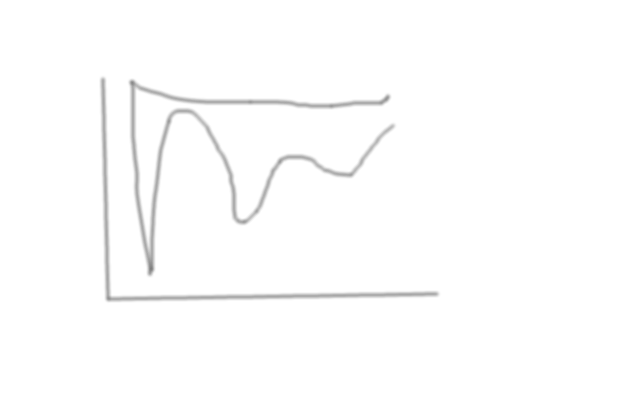
\includegraphics[width=0.8\columnwidth]{./pix/tmp.png}
  \caption{The commanded reference plotted against the actual reference recorded via Hubo-Ach and ground truth via CAN analyzing utilities.  In this plot the commanded reference is automatically filtered by Hubo-Ach.}
  \label{fig:singleJointStepFiltered}
\end{figure}

\begin{figure}[thpb]
  \centering
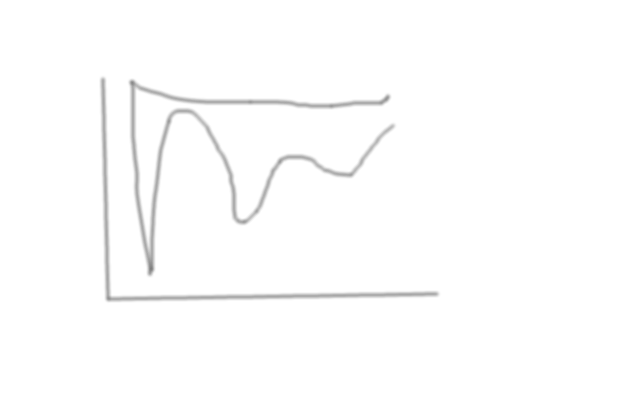
\includegraphics[width=0.8\columnwidth]{./pix/tmp.png}
  \caption{$\theta_r$ plotted against $\theta_c$ and $\theta_a$ recorded via Hubo-Ach with values for $L$ ranging from 1 to 200.}
  \label{fig:singleJointStepFilteredLtest}
\end{figure}

This method is a feed-forward method that assumes that the position you set the actuator to is the actual position of the actuator.

	\subsection{Compliance Amplification}\label{sec:singlejointRefComplience}
		Compliance amplification takes advandage of the internal compliance of the joints and amplifies that by feeding back the PID error $\theta_e$.
Like the Equation~\ref{eq:refrefmode} we have no past information about the set reference and we have only the compiliance given by the joints.
If we think about $\theta_e$ and what effects it we can use it to add compliance to our system.
It is important to note that because the Hubo is a high-gain PID position controlled device with an intergral gain $K_i$ set to zero the steady state error of the joint (the PID error $\theta_e$) is proportional to the moment applied to the joint.
If we combine the reference $\theta_r$ and $\theta_e$ multiplied by a compliance gain $K_c$ we are able to add/amplify the compliance to the system.

\begin{equation}
\theta_c(N) = K_c\theta_e(N)+\theta_r(N)
\end{equation}

It is important to note that $K_c \leq 1$ or the system will go unstable.
If $K_c=1$ then we have

\begin{equation}
\theta_c(N) = \theta_a(N)
\end{equation}

	\subsection{Joint Space Step Response with Feedback Filtering}\label{sec:singlejointEnc}
		Feedback filtering allows us to removes the requirement that we know the joint's current position.
Similar to Equation~\ref{eq:reffiltermode} this method sets $\theta_c$ based on a filter length $L$ and the current desired value $\theta_r$.
However instead of assuming that we know all past $\theta_r$ we use the actual position $\theta_a$.
This method add compliance in a similar way to that of Section~\ref{sec:singlejointRefComplience}.


\begin{equation}\label{eq:refencmode}
\theta_c(N) = \frac{\theta_a(N)\cdot\left(L-1\right) + \theta_r(N)}{L}
\end{equation}

This causes three major effects: 

\noindent \textbf{Effect 1:} The movement of the joint is guaranteed to be filtered even if the previous reference is unknown.

\noindent \textbf{Effect 2:} The steady state error of the feedback filtering method $\theta_e^{fbfilter}$ is greater than that of the PID error $\theta_e$ in the direction of the moment acting on the joint.

\begin{equation}
\theta_e^{fbfilter} > \theta_e
\end{equation}

\noindent \textbf{Effect 3:} The joint's compliance has increased due to the effect of the moment applied to the joint has on the steady state error.

\begin{figure}
\centering

\begin{tikzpicture}[->,>=stealth',shorten >=1pt,auto,node distance=5cm,
  thick,main node/.style={fill=white!20,draw,font=\sffamily\Large\bfseries}]


  \node[main node] (ref) {Reference};
  \node[main node] (filter) [right=3.0cm of ref] {Filter};
  \node[main node] (hubo-ach) [below=1.0cm of filter] {Hubo-Ach};
  \node[main node] (hubo) [right=3.0cm of hubo-ach] {Hubo};




  \path[<->,dashed, every node/.style={font=\sffamily\small}]
    (hubo) edge node [above] {CAN} (hubo-ach);

  \path[->,every node/.style={font=\sffamily\small}]
    (ref) edge node [above] {$\theta_d$} (filter);

  \path[->,every node/.style={font=\sffamily\small}]
    (hubo-ach) edge node [left] {$\theta_r$} (filter);

  \path[->,every node/.style={font=\sffamily\small}]
    (filter) edge node [right] {$\theta_a$} (hubo-ach);


% look into this and add z^-1

\path [every node/.style={draw,minimum width=3cm, minimum height=5cm]}]
  node (a) at (0,0) {}
  [xshift=7cm]
  node (b) at (0,0) {}
  [xshift=7cm]
  node (c) at (0,0) {};

%\begin{scope}[->,>=latex]
%    \foreach \i in {-2,...,2}{% 
%      \draw[->] ([yshift=\i * 0.8 cm]a.east) -- ([yshift=\i * 0.8 cm]b.west) ;}

%    \foreach \i in {1,2}{% 
%      \draw[->] ([yshift=\i * 0.8 cm]a.east) to [out=50,in=130] ([yshift=\i * 0.8 cm]c.west) ;} 

%    \foreach \i in {-1,-2}{% 
%      \draw[->] ([yshift=\i * 0.8 cm]a.east) to [out=-50,in=-130] ([yshift=\i * 0.8 cm]c.west) ;}
%\end{scope}


\end{tikzpicture}
\caption{Desired reference $\theta_d$ being filtered before applied to Hubo via Hubo-Ach.  $\theta_d$ is sent through a filter that reduces the \textit{jerk} on the actuator then the new reference $\theta_r$ is set on the \textbf{FeedForward} channel, Hubo-Ach reads it then commands Hubo at the rising edge of the next cycle.}
\label{fig:hubo-ach-feedforward}
\end{figure}



Fig.~\ref{fig:singleJointStepFilteredFeedback} shows $\theta_r$ plotted against $\theta_c$ and $\theta_a$.  
$\theta_a$ not only lags behind $\theta_c$ but it also has a greater steady state error.
Fig.~\ref{fig:singleJointStepFilteredFeedbackMoment} shows how the steady state error $\theta_e^{fbfilter}$ increases with an applied moment.
This is where we get our compliance.

\begin{figure}[thpb]
  \centering
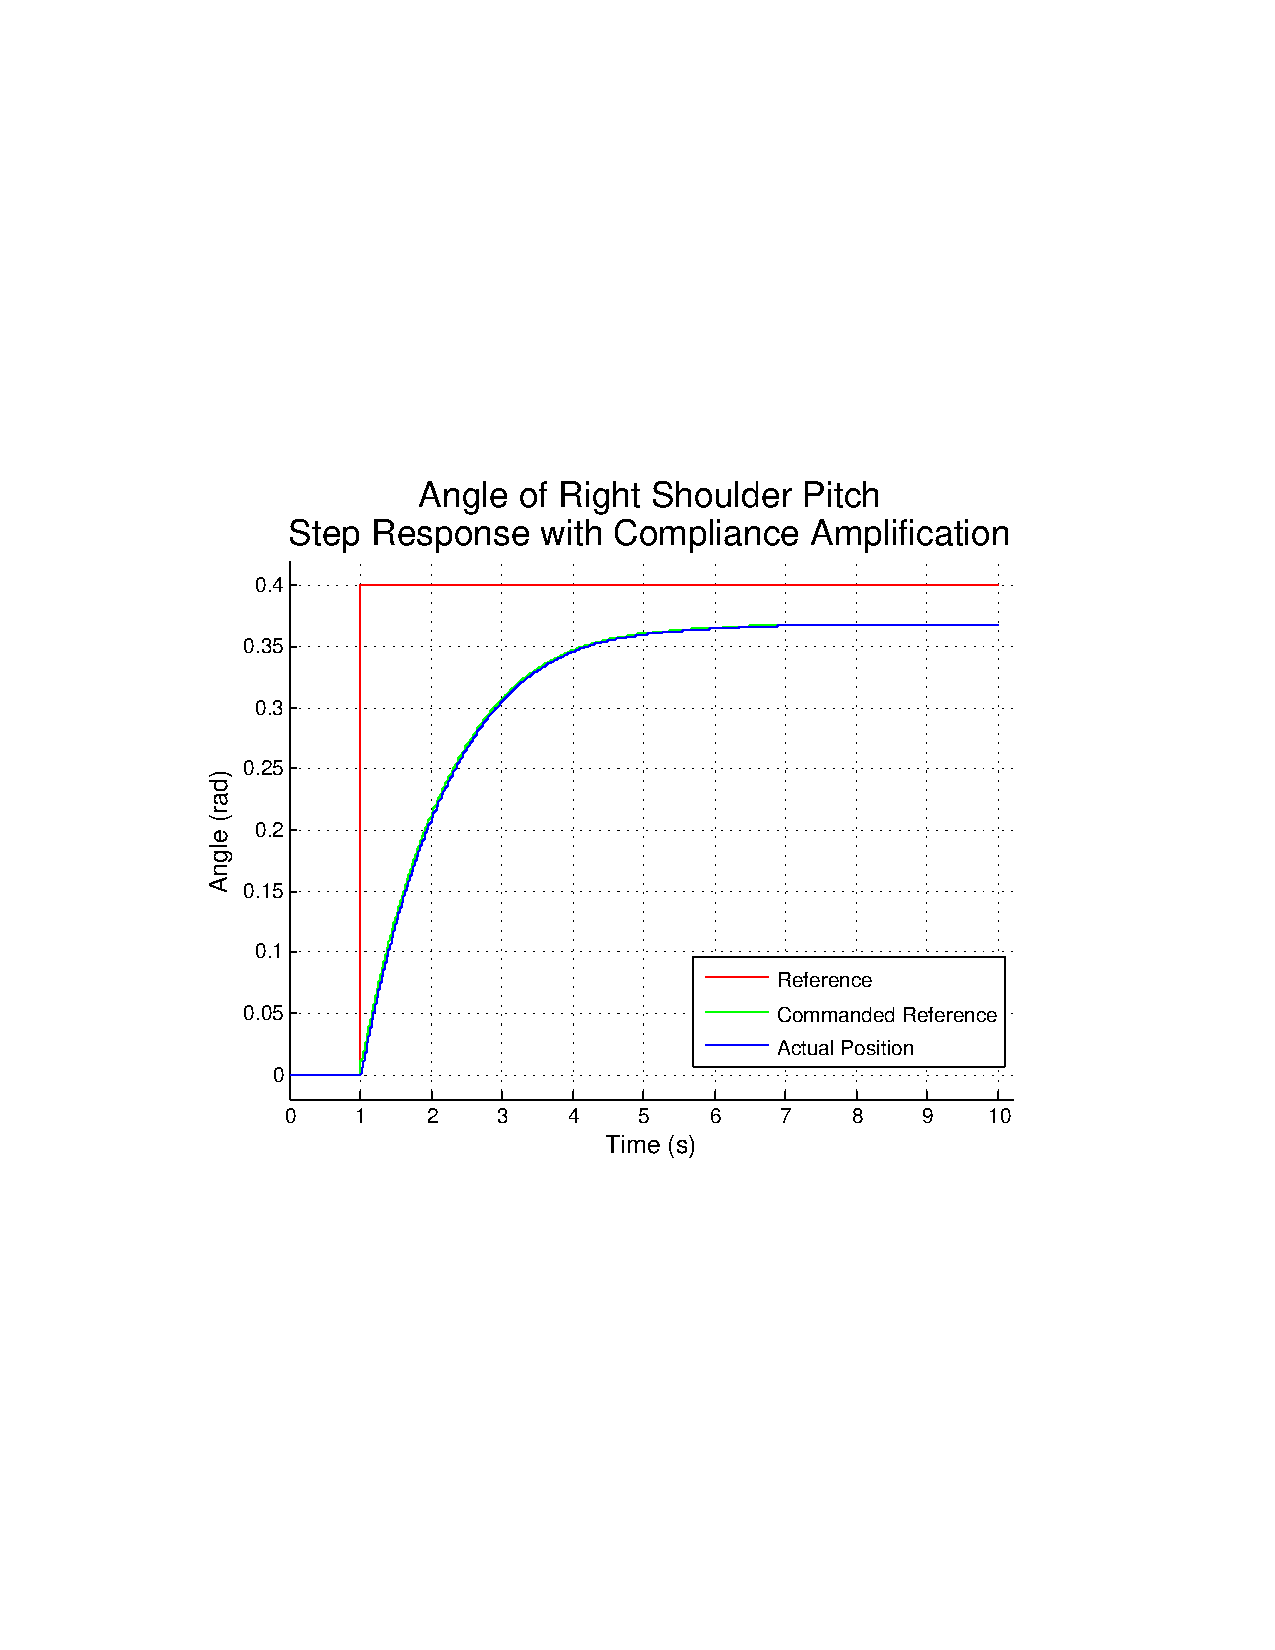
\includegraphics[width=0.8\columnwidth]{./examples/pix/RSP-Zp4-step-enc-real-crop.pdf}
  \caption{$\theta_r$ plotted against $\theta_c$ and $\theta_a$ recorded via Hubo-Ach using the feedback filtering method.}
  \label{fig:singleJointStepFilteredFeedback}
\end{figure}

\begin{figure}[thpb]
  \centering
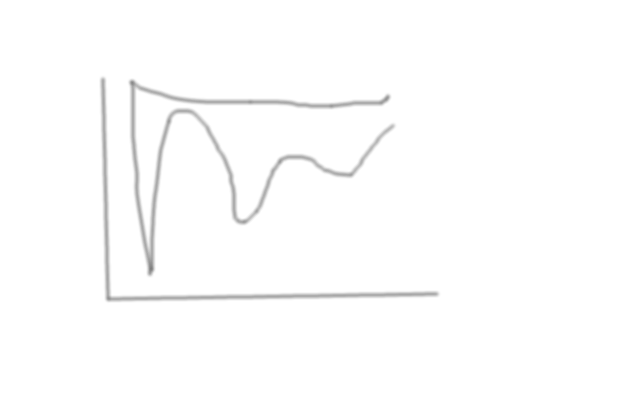
\includegraphics[width=0.8\columnwidth]{./pix/tmp.png}
  \caption{$\theta_r$ plotted against $\theta_c$ and $\theta_a$ recorded via Hubo-Ach using the feedback filtering method with different moments applied to the joint.  You will note that as the moment increases so does $\theta_e^{fbfilter}$. }
  \label{fig:singleJointStepFilteredFeedbackMoment}
\end{figure}

\section{Six Degree of Freedom Inverse Kinimatic Implimentation Example}\label{sec:6dofik}
This section shows how we calculate the inverse kinimatics (IK) for the Hubo's right arm and how we use that calculation in conjunction with Section~\ref{sec:simpleExamples}.  The result is the ability to command the end effector (EEF)
	\subsection{Work Space Controller Example}
		The next step is to find the inverse kinematic (IK) solution for the right arm.
Inherently this problem has multiple solutions.
When solving the IK Pieper\cite{peiper1968kinematics} states that a closed-form solution does exist if:
\begin{itemize}
\item Three consecutive joints axes of the manipulator are parallel to one another
\end{itemize}

OR
\begin{itemize}
\item Three consecutive joints intercect at a single point
\end{itemize}

The kinematic structure in Fig~\ref{fig:hubo} and Fig~\ref{fig:IkFkCoordinate} shows that the Hubo2+ platform does have a three joints that intersect the same point in the shoulders and in the hips.
Thus a closed-form solution exists for both arms and both legs.

The transform $T_0^6$ in Equation~\ref{eq:t06} is needed to solve the IK problem for the shoulder.  
It is important to note that $T_0^6$ is in the form of

\begin{equation}\label{eq:T06}
T_0^6 = \left[ \begin{array}{cccc} 
\overline{x_6} & \overline{y_6} & \overline{z_6} & \overline{p_6} \\
0              & 0              & 0              & 1   
\end{array} \right]
\end{equation} 

Where $\overline{x_6}$, $\overline{y_6}$ and $\overline{z_6}$ are $[3x1]$ unit vectors along the principle axes of the end-effectors coordinate frame $i$, see Fig.~\ref{fig:IkFkCoordinate}.
Position vector $\overline{p_6}$ describes the hand about joint $A1$ (shoulder).
The arm can be vied in different frames.
If we look at the arm in reference to the end-effector's frame.
The reverse transform is defined as $(T_0^6)`$


\begin{equation}
(T_0^6)' = T_6^0 = (T_0^6)^{-1} = \left[ \begin{array}{cccc} 
\overline{x_6} & \overline{y_6} & \overline{z_6} & \overline{p_6} \\
0              & 0              & 0              & 1   
\end{array} \right]^{-1}
\end{equation} 

The following method is based on the work done by our partner Park et. al.\cite{5649842}.
The general link translation matrix $T_{i-1}^i$ relates the $i^{th}$ coordinate frame to the $(i-1)^{th}$ coordinate frame.  
In addition we can extend Equation~\ref{eq:T06} to

\begin{equation}\label{eq:06invIK}
T_0^6 = \left[ \begin{array}{cccc} 
\overline{x_6} & \overline{y_6} & \overline{z_6} & \overline{p_6} \\
0              & 0              & 0              & 1   
\end{array} \right] = \left[ \begin{array}{cccc} 
\overline{n} & \overline{s} & \overline{a} & \overline{p} \\
0            & 0            & 0            & 1   
\end{array} \right]
\end{equation} 

Where $[\overline{n}, \overline{s}, \overline{a}, \overline{p}]$ represents the normal vector, the sliding vector, the approach vector and the position vector of the end effector respectively\cite{fu1987robotics}.  We can now state that

\begin{equation}
(T_0^6)' = T_6^0 = (T_0^6)^{-1} = \left[ \begin{array}{cccc} 
\overline{x_6} & \overline{y_6} & \overline{z_6} & \overline{p_6} \\
0              & 0              & 0              & 1   
\end{array} \right]^{-1}= \left[ \begin{array}{cccc} 
\overline{n}' & \overline{s}' & \overline{a}' & \overline{p}' \\
0             & 0             & 0             & 1   
\end{array} \right]
\end{equation} 

We can now use the reverse method to solve for the joint angles as in \cite{fu1987robotics} and derived in the tech report\cite{gtechIK2}.
The first three lower joint angles of $A_4$, $A_5$ and $A_6$ are solved for.
Subsequently the upper joint angles of $A_1$, $A_2$ and $A_3$ are solved.

Using inverse transform methods\cite{4046335} we can modify Equation~\ref{eq:t06} to

\begin{equation}\label{eq:t06IK}
T_6^0 = (T_0^6)^{-1} = \prod_{i=6}^{1} T_{i}^{i-1} = T_{6}^{5}T_{5}^{4}T_{4}^{3}T_{3}^{2}T_{2}^{1}T_{1}^{0}
\end{equation}

Then we equate Equation~\ref{eq:06invIK} to Equation~\ref{eq:t06IK} 

\begin{equation}
T_{6}^{5}T_{5}^{4}T_{4}^{3}T_{3}^{2}T_{2}^{1}T_{1}^{0} = \left[ \begin{array}{cccc} 
\overline{n}' & \overline{s}' & \overline{a}' & \overline{p}' \\
0             & 0             & 0             & 1   
\end{array} \right]
\end{equation}

Then move $T_6^5$ to the other side of the equation


\begin{equation}\label{eq:preG}
T_{5}^{4}T_{4}^{3}T_{3}^{2}T_{2}^{1}T_{1}^{0} = T_{5}^{6}\left[ \begin{array}{cccc} 
\overline{n}' & \overline{s}' & \overline{a}' & \overline{p}' \\
0             & 0             & 0             & 1   
\end{array} \right]
\end{equation}

For simplicity we will represent Equation~\ref{eq:preG} as $G_L$ and $G_R$ standing for \textit{right} and \textit{left} side.

\begin{equation}
G_L = T_{5}^{6}\left[ \begin{array}{cccc} 
\overline{n}' & \overline{s}' & \overline{a}' & \overline{p}' \\
0             & 0             & 0             & 1   
\end{array} \right]
\end{equation}



\begin{equation}
G_R = T_{5}^{4}T_{4}^{3}T_{3}^{2}T_{2}^{1}T_{1}^{0} 
\end{equation}


Expanding gives us

\begin{equation}
G_L = \left[ \begin{array}{cccc} 
g_{11} & g_{12} & g_{13} & cos(\theta_6)(p_x'+l_{A_4})-sin(\theta_6)p_y' \\
g_{21} & g_{22} & g_{23} & sin(\theta_6)(p_x'+l_{A_4})-cos(\theta_6)p_y' \\
g_{31} & g_{32} & g_{33} & p_z'                                         \\
0      & 0      & 0      & 1   
\end{array} \right]
\end{equation}

and

\begin{equation}
G_R = \left[ \begin{array}{cccc} 
g_{11} & g_{12} & g_{13} & sin(\theta_4)cos(\theta_5)l_{A_2} \\
g_{21} & g_{22} & g_{23} & -cos(\theta_6)l_{A_2}-l_{A3}       \\
g_{31} & g_{32} & g_{33} & sin(\theta_4)sin(\theta_5)l_{A_2}  \\
0      & 0      & 0      & 1   
\end{array} \right]
\end{equation}

We can then equate elements $(1,4)$, $(2,4)$ and $(3,4)$ of $G_L$ and $G_R$. 
This gives us

\begin{equation}\label{eq:thetaSolve11}
cos(\theta_6)(p_x'+l_{A_4})-sin(\theta_6)p_y' = sin(\theta_4)cos(\theta_5)l_{A_2}
\end{equation}

\begin{equation}\label{eq:thetaSolve12}
sin(\theta_6)(p_x'+l_{A_4})-cos(\theta_6)p_y' = -cos(\theta_6)l_{A_2}-l_{A3}
\end{equation}

\begin{equation}\label{eq:thetaSolve13}
p_z' = sin(\theta_4)sin(\theta_5)l_{A_2}
\end{equation}

Based on the desired task space location we let

\begin{equation}\label{eq:thetaSolve21}
p_x' + l_{A_4} = r \cdot cos(\phi)
\end{equation}

and

\begin{equation}\label{eq:thetaSolve22}
p_y' = r \cdot sin(\phi)
\end{equation}

where 

\begin{equation}\label{eq:thetaSolve31}
r = sqrt{(p_x'+l_{A_4})^2 + (p_y')^2}
\end{equation}

and 

\begin{equation}\label{eq:thetaSolve32}
\phi = atan2(p_y',p_x'+l_{A_4})
\end{equation}

\textbf{Note:} $atan2()$ represents the the $atan$ method that gathers the information of the signs of the inputs in order to put the returned value in the appropriate quadrant.

Combining Equation (\ref{eq:thetaSolve11}), (\ref{eq:thetaSolve12}) and (\ref{eq:thetaSolve13}) with Equation (\ref{eq:thetaSolve21}) and (\ref{eq:thetaSolve22}) we get

\begin{equation}\label{eq:thetaSolve41}
r \cdot cos(\theta_6+\phi) = sin(\theta_4)cos(\theta_5)l_{A_2}
\end{equation}

\begin{equation}\label{eq:thetaSolve42}
r \cdot sin(\theta_6+\phi) = -cos(\theta_4)l_{A_2}-l_{A_3}
\end{equation}

\begin{equation}\label{eq:thetaSolve43}
p_z' = sin(\theta_4)sin(\theta_5)l_{A_2}
\end{equation}


When we combine above with Equation (\ref{eq:thetaSolve31}) and (\ref{eq:thetaSolve32}) and obtain 


\begin{equation}
\theta_4 = atan2\left( \pm \sqrt{1-cos(\theta_4)^2} , cos(\theta_4)  \right)
\end{equation}

where

\begin{equation}
cos(\theta_4) = \frac{(p_x'+l_{A_4})^2  +  p_y'^2  +  p_z'^2  -  l_{A_2}^2  -  l_{A_3}^2}
                     {2l_{A_2}l_{A3}}
\end{equation}

Using Equation~\ref{eq:thetaSolve43} we can get $\theta_5$

\begin{equation}
\theta_5 = atan2(sin(\theta_5), \pm\sqrt{1-sin(\theta_5)^2})
\end{equation}

where

\begin{equation}
sin(\theta_5) = \frac{p_z'}
                     {sin(\theta_4)l_{A_2}}
\end{equation}


We can then solve for $\theta_6$ by dividing Equation~\ref{eq:thetaSolve42} by Equation~\ref{eq:thetaSolve41}.



\begin{equation}
\frac{r \cdot sin(\theta_6+\phi)}
     {r \cdot cos(\theta_6+\phi)} = tan(\theta_6+\phi) = \frac{-cos(\theta_4)l_{A_2}-l_{A_3}}
                                                              {sin(\theta_4)cos(\theta_5)l_{A_2}}
\end{equation}

\begin{equation}
\theta_6 = atan2(-(cos(\theta_4)l_{A_2}+l_{A_3}), sin(\theta_4)cos(\theta_5)l_{A_2}) - \phi
\end{equation}


	\subsection{Six DOF IK Implimentaiton}
		In order to control the Hubo's upper body manipulators in work space as opposed to joint space both forward and inverse kinematics are required, (FK) and (IK) respectively.
In order to find a proper solution the joint limits, singularities and feasible workspace (no-self collisions) must be accounted for.

The kinematic structure of the right and left arm of the Hubo are identical with the caveat that the work space offset is mirrored over the z-axis.
This means that they have the same Denavit–Hartenberg (DH) parameters.

\begin{table}
\centering
\caption{Denavit–Hartenberg for Hubo2+ upper body (arms) in standard format}
\begin{tabular}{|l | c|}
\hline
Link     & Length (m) \\
\hline
\hline
$l_{A1}$ & 0.215 \\
\hline
$l_{A2}$ & 0.179 \\
\hline
$l_{A3}$ & 0.182 \\
\hline
$l_{A4}$ & 0.121 \\
\hline
$l_{E}$ & 0.100 \\

\hline

\end{tabular}\label{table:DHupper}
\end{table}

\begin{figure}
\centering

\begin{tikzpicture}[->,>=stealth',shorten >=1pt,auto,node distance=5cm,
  thick,main node/.style={fill=white!20,draw,font=\sffamily\small\bfseries}]

  \node[main node] (ref) [text width=3cm] {End Effector Position};

  \node[main node] (ik) [right=2.0cm of ref] {6-DOF IK};
  \node[main node] (filter) [right=2.0cm of ik] {Filter};
  \node[main node] (hubo-ach) [below=1.0cm of filter] {Hubo-Ach};
  \node[main node] (hubo) [right=2.0cm of hubo-ach] {Hubo};



  \path[->, every node/.style={font=\sffamily\small}]
    (ref) edge node [above] {$(x,y,z)$} (ik)
    (ref) edge node [below] {$(\alpha,\beta,\gamma)$} (ik);
%  \path[->, every node/.style={font=\sffamily\small}]
%    (ref) edge node [below] {$(\alpha,\beta,\gamma)$} (ik);

 

  \path[->,every node/.style={font=\sffamily\small}]
    (ik) edge node [above] {$\overline{\theta_d}$} (filter);

 \draw[->] ([xshift=-0.5 cm]filter.south)  -- node [left] {$\overline{\theta_r}$} ([xshift=-0.5 cm]hubo-ach.north)  ;
 \draw[->] ([xshift=0.5 cm]hubo-ach.north) -- node [left] {$\overline{\theta_a}$} ([xshift=0.5 cm]filter.south)  ;

 \path[<->,dashed, every node/.style={font=\sffamily\small}]
    (hubo) edge node [above] {CAN} (hubo-ach);

%  \path[->,every node/.style={font=\sffamily\small}]
%    (hubo-ach) edge node [left] {$\theta_r$} (filter);

%  \path[->,every node/.style={font=\sffamily\small}]
%    (filter) edge node [right] {$\theta_a$} (hubo-ach);




% look into this and add z^-1

%\path [every node/.style={draw,minimum width=3cm, minimum height=5cm]}]
%  node (a) at (0,0) {}
%  [xshift=7cm]
%  node (b) at (0,0) {}
%  [xshift=7cm]
%  node (c) at (0,0) {};

%\begin{scope}[->,>=latex]
%    \foreach \i in {-2,...,2}{% 
%      \draw[->] ([yshift=\i * 0.8 cm]a.east) -- ([yshift=\i * 0.8 cm]b.west) ;}

%    \foreach \i in {1,2}{% 
%      \draw[->] ([yshift=\i * 0.8 cm]a.east) to [out=50,in=130] ([yshift=\i * 0.8 cm]c.west) ;} 

%    \foreach \i in {-1,-2}{% 
%      \draw[->] ([yshift=\i * 0.8 cm]a.east) to [out=-50,in=-130] ([yshift=\i * 0.8 cm]c.west) ;}
%\end{scope}


\end{tikzpicture}
\caption{Desired reference $\theta_d$ being filtered before applied to Hubo via Hubo-Ach.  $\theta_d$ is sent through a filter that reduces the \textit{jerk} on the actuator by using Equation~\ref{eq:refencmode}.  The new reference $\theta_r$ is set on the \textbf{FeedForward} channel, Hubo-Ach reads it then commands Hubo at the rising edge of the next cycle.  This method adds compliance to the system}
\label{fig:hubo-ach-feedforwardFilterFeedBack}
\end{figure}



		\subsubsection{Froward Kinematics} 
			The transform between joint adjacent joints is represented by the transform:

\begin{equation}
T_i^{i-1} = \left[ \begin{array}{cccc} 
cos(\theta_i) & -sin(\theta_i)cos(\alpha_i) &  sin(\theta_i)sin(\alpha_i)  &  a_i cos(\theta_i) \\ 
sin(\theta_i) &  cos(\theta_i)cos(\alpha_i) & -cos(\theta_i)sin(\alpha_i)  &  a_i sin(\theta_i) \\
0             &  sin(\alpha_i)              &  cos(\alpha_i)               &  d_i               \\
0             &  0                          &  0                           &  1                 
\end{array} \right]
\end{equation}

Where $\theta_i$ is the 

\begin{figure}[thpb]
  \centering
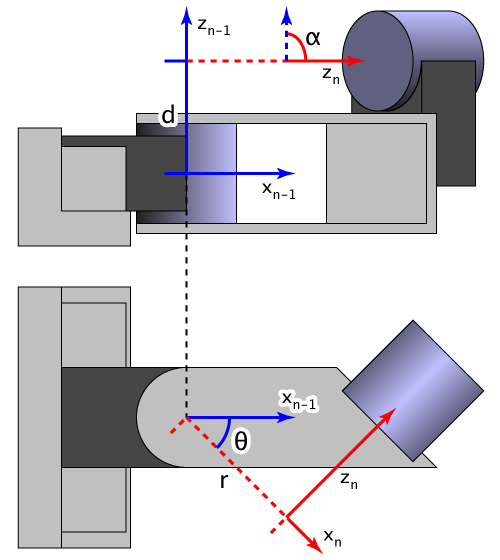
\includegraphics[width=0.8\columnwidth]{./examples/pix/Sample_Denavit-Hartenberg_Diagram.png}

		\subsubsection{Inverse Kinematics}
			The next step is to find the inverse kinematic (IK) solution for the right arm.
Inherently this problem has multiple solutions.
When solving the IK Pieper\cite{peiper1968kinematics} states that a closed-form solution does exist if:
\begin{itemize}
\item Three consecutive joints axes of the manipulator are parallel to one another
\end{itemize}

OR
\begin{itemize}
\item Three consecutive joints intercect at a single point
\end{itemize}

The kinematic structure in Fig~\ref{fig:hubo} and Fig~\ref{fig:IkFkCoordinate} shows that the Hubo2+ platform does have a three joints that intersect the same point in the shoulders and in the hips.
Thus a closed-form solution exists for both arms and both legs.

The transform $T_0^6$ in Equation~\ref{eq:t06} is needed to solve the IK problem for the shoulder.  
It is important to note that $T_0^6$ is in the form of

\begin{equation}\label{eq:T06}
T_0^6 = \left[ \begin{array}{cccc} 
\overline{x_6} & \overline{y_6} & \overline{z_6} & \overline{p_6} \\
0              & 0              & 0              & 1   
\end{array} \right]
\end{equation} 

Where $\overline{x_6}$, $\overline{y_6}$ and $\overline{z_6}$ are $[3x1]$ unit vectors along the principle axes of the end-effectors coordinate frame $i$, see Fig.~\ref{fig:IkFkCoordinate}.
Position vector $\overline{p_6}$ describes the hand about joint $A1$ (shoulder).
The arm can be vied in different frames.
If we look at the arm in reference to the end-effector's frame.
The reverse transform is defined as $(T_0^6)`$


\begin{equation}
(T_0^6)' = T_6^0 = (T_0^6)^{-1} = \left[ \begin{array}{cccc} 
\overline{x_6} & \overline{y_6} & \overline{z_6} & \overline{p_6} \\
0              & 0              & 0              & 1   
\end{array} \right]^{-1}
\end{equation} 

The following method is based on the work done by our partner Park et. al.\cite{5649842}.
The general link translation matrix $T_{i-1}^i$ relates the $i^{th}$ coordinate frame to the $(i-1)^{th}$ coordinate frame.  
In addition we can extend Equation~\ref{eq:T06} to

\begin{equation}\label{eq:06invIK}
T_0^6 = \left[ \begin{array}{cccc} 
\overline{x_6} & \overline{y_6} & \overline{z_6} & \overline{p_6} \\
0              & 0              & 0              & 1   
\end{array} \right] = \left[ \begin{array}{cccc} 
\overline{n} & \overline{s} & \overline{a} & \overline{p} \\
0            & 0            & 0            & 1   
\end{array} \right]
\end{equation} 

Where $[\overline{n}, \overline{s}, \overline{a}, \overline{p}]$ represents the normal vector, the sliding vector, the approach vector and the position vector of the end effector respectively\cite{fu1987robotics}.  We can now state that

\begin{equation}
(T_0^6)' = T_6^0 = (T_0^6)^{-1} = \left[ \begin{array}{cccc} 
\overline{x_6} & \overline{y_6} & \overline{z_6} & \overline{p_6} \\
0              & 0              & 0              & 1   
\end{array} \right]^{-1}= \left[ \begin{array}{cccc} 
\overline{n}' & \overline{s}' & \overline{a}' & \overline{p}' \\
0             & 0             & 0             & 1   
\end{array} \right]
\end{equation} 

We can now use the reverse method to solve for the joint angles as in \cite{fu1987robotics} and derived in the tech report\cite{gtechIK2}.
The first three lower joint angles of $A_4$, $A_5$ and $A_6$ are solved for.
Subsequently the upper joint angles of $A_1$, $A_2$ and $A_3$ are solved.

Using inverse transform methods\cite{4046335} we can modify Equation~\ref{eq:t06} to

\begin{equation}\label{eq:t06IK}
T_6^0 = (T_0^6)^{-1} = \prod_{i=6}^{1} T_{i}^{i-1} = T_{6}^{5}T_{5}^{4}T_{4}^{3}T_{3}^{2}T_{2}^{1}T_{1}^{0}
\end{equation}

Then we equate Equation~\ref{eq:06invIK} to Equation~\ref{eq:t06IK} 

\begin{equation}
T_{6}^{5}T_{5}^{4}T_{4}^{3}T_{3}^{2}T_{2}^{1}T_{1}^{0} = \left[ \begin{array}{cccc} 
\overline{n}' & \overline{s}' & \overline{a}' & \overline{p}' \\
0             & 0             & 0             & 1   
\end{array} \right]
\end{equation}

Then move $T_6^5$ to the other side of the equation


\begin{equation}\label{eq:preG}
T_{5}^{4}T_{4}^{3}T_{3}^{2}T_{2}^{1}T_{1}^{0} = T_{5}^{6}\left[ \begin{array}{cccc} 
\overline{n}' & \overline{s}' & \overline{a}' & \overline{p}' \\
0             & 0             & 0             & 1   
\end{array} \right]
\end{equation}

For simplicity we will represent Equation~\ref{eq:preG} as $G_L$ and $G_R$ standing for \textit{right} and \textit{left} side.

\begin{equation}
G_L = T_{5}^{6}\left[ \begin{array}{cccc} 
\overline{n}' & \overline{s}' & \overline{a}' & \overline{p}' \\
0             & 0             & 0             & 1   
\end{array} \right]
\end{equation}



\begin{equation}
G_R = T_{5}^{4}T_{4}^{3}T_{3}^{2}T_{2}^{1}T_{1}^{0} 
\end{equation}


Expanding gives us

\begin{equation}
G_L = \left[ \begin{array}{cccc} 
g_{11} & g_{12} & g_{13} & cos(\theta_6)(p_x'+l_{A_4})-sin(\theta_6)p_y' \\
g_{21} & g_{22} & g_{23} & sin(\theta_6)(p_x'+l_{A_4})-cos(\theta_6)p_y' \\
g_{31} & g_{32} & g_{33} & p_z'                                         \\
0      & 0      & 0      & 1   
\end{array} \right]
\end{equation}

and

\begin{equation}
G_R = \left[ \begin{array}{cccc} 
g_{11} & g_{12} & g_{13} & sin(\theta_4)cos(\theta_5)l_{A_2} \\
g_{21} & g_{22} & g_{23} & -cos(\theta_6)l_{A_2}-l_{A3}       \\
g_{31} & g_{32} & g_{33} & sin(\theta_4)sin(\theta_5)l_{A_2}  \\
0      & 0      & 0      & 1   
\end{array} \right]
\end{equation}

We can then equate elements $(1,4)$, $(2,4)$ and $(3,4)$ of $G_L$ and $G_R$. 
This gives us

\begin{equation}\label{eq:thetaSolve11}
cos(\theta_6)(p_x'+l_{A_4})-sin(\theta_6)p_y' = sin(\theta_4)cos(\theta_5)l_{A_2}
\end{equation}

\begin{equation}\label{eq:thetaSolve12}
sin(\theta_6)(p_x'+l_{A_4})-cos(\theta_6)p_y' = -cos(\theta_6)l_{A_2}-l_{A3}
\end{equation}

\begin{equation}\label{eq:thetaSolve13}
p_z' = sin(\theta_4)sin(\theta_5)l_{A_2}
\end{equation}

Based on the desired task space location we let

\begin{equation}\label{eq:thetaSolve21}
p_x' + l_{A_4} = r \cdot cos(\phi)
\end{equation}

and

\begin{equation}\label{eq:thetaSolve22}
p_y' = r \cdot sin(\phi)
\end{equation}

where 

\begin{equation}\label{eq:thetaSolve31}
r = sqrt{(p_x'+l_{A_4})^2 + (p_y')^2}
\end{equation}

and 

\begin{equation}\label{eq:thetaSolve32}
\phi = atan2(p_y',p_x'+l_{A_4})
\end{equation}

\textbf{Note:} $atan2()$ represents the the $atan$ method that gathers the information of the signs of the inputs in order to put the returned value in the appropriate quadrant.

Combining Equation (\ref{eq:thetaSolve11}), (\ref{eq:thetaSolve12}) and (\ref{eq:thetaSolve13}) with Equation (\ref{eq:thetaSolve21}) and (\ref{eq:thetaSolve22}) we get

\begin{equation}\label{eq:thetaSolve41}
r \cdot cos(\theta_6+\phi) = sin(\theta_4)cos(\theta_5)l_{A_2}
\end{equation}

\begin{equation}\label{eq:thetaSolve42}
r \cdot sin(\theta_6+\phi) = -cos(\theta_4)l_{A_2}-l_{A_3}
\end{equation}

\begin{equation}\label{eq:thetaSolve43}
p_z' = sin(\theta_4)sin(\theta_5)l_{A_2}
\end{equation}


When we combine above with Equation (\ref{eq:thetaSolve31}) and (\ref{eq:thetaSolve32}) and obtain 


\begin{equation}
\theta_4 = atan2\left( \pm \sqrt{1-cos(\theta_4)^2} , cos(\theta_4)  \right)
\end{equation}

where

\begin{equation}
cos(\theta_4) = \frac{(p_x'+l_{A_4})^2  +  p_y'^2  +  p_z'^2  -  l_{A_2}^2  -  l_{A_3}^2}
                     {2l_{A_2}l_{A3}}
\end{equation}

Using Equation~\ref{eq:thetaSolve43} we can get $\theta_5$

\begin{equation}
\theta_5 = atan2(sin(\theta_5), \pm\sqrt{1-sin(\theta_5)^2})
\end{equation}

where

\begin{equation}
sin(\theta_5) = \frac{p_z'}
                     {sin(\theta_4)l_{A_2}}
\end{equation}


We can then solve for $\theta_6$ by dividing Equation~\ref{eq:thetaSolve42} by Equation~\ref{eq:thetaSolve41}.



\begin{equation}
\frac{r \cdot sin(\theta_6+\phi)}
     {r \cdot cos(\theta_6+\phi)} = tan(\theta_6+\phi) = \frac{-cos(\theta_4)l_{A_2}-l_{A_3}}
                                                              {sin(\theta_4)cos(\theta_5)l_{A_2}}
\end{equation}

\begin{equation}
\theta_6 = atan2(-(cos(\theta_4)l_{A_2}+l_{A_3}), sin(\theta_4)cos(\theta_5)l_{A_2}) - \phi
\end{equation}














\section{Simulator}\label{sec:simulator}
This section discribes how the system connects with a simulator 


\section{Task}\label{sec:task}
Turning a valve with whole body (more of a lever)
\begin{itemize}
\item Find the valve - sensing
\item Move to the valve - close loop on sensing
\item Grab the valve
\item Jump on the valve
\end{itemize}



\section{System setup}

State diagram of plan
\begin{itemize}
\item Find the valve - sensing
\item Move to the valve - close loop on sensing
\item Grab the valve
\item Jump on the valve
\end{itemize}

Software structrue
\begin{itemize}
\item Hubo-Ach
\item ROS (the connectiving with latency/non-real time problem)

\item Etc.
\end{itemize}


Sensors Chosen
\begin{itemize}
\item FT
\item IMU
\item Monocular
\item RGB-D
\end{itemize}

Controllers
\begin{itemize}
\item Walking
\item Balance
\item Complience
\item IK
\item Visual Servoing
\end{itemize}

\section{Results}\label{sec:results}
\begin{itemize}
\item What worked
\item What did not
\item To be improved
\end{itemize}
